\section{Results}\label{results}
In this section we describe the results.


\subsection{Matlab 3D plots}
To prove the functions of the algorithm provided in section \ref{section:depthmap}, MATLAB was used to make a 3D plot of the fish. (See figure \ref{fig:3D_plot_63} and \ref{fig:3D_plot_87}). From these plots it is easy to see the differences from the original depthmap to the enhanced depthmap. The totalfocus image is put on top of the enhanced depthmap to make it even clearer that the resulting contour has nearly the same contour as the actual fish. It is also seen that most particles are removed, and the surface of the fish is evened out.

Still, some errors remain. The contour of the fish is not exact, and some pixels on the border of the fish has git the wrong value. To find the contour, some eroding and dilating is used, and this can result in a contour that is not exact. To get the contour not to leave out larger areas of the fishes belly, this eroding and dilating is needed, so the contour is within reason. What concern the pixels surrounding the border of the fish, is some wrong measurements by the Raytrix, and other is particles on the border with close depthmap color to the rest of the fish. It looks like many particles in the 3D plot, but it is actually just about 10-20 single pixels in total in an image, so the biomass estimation will not get significantly affected.  


\begin{figure}[H]
    \centering
    \begin{subfigure}{1\textwidth}
        \centering
        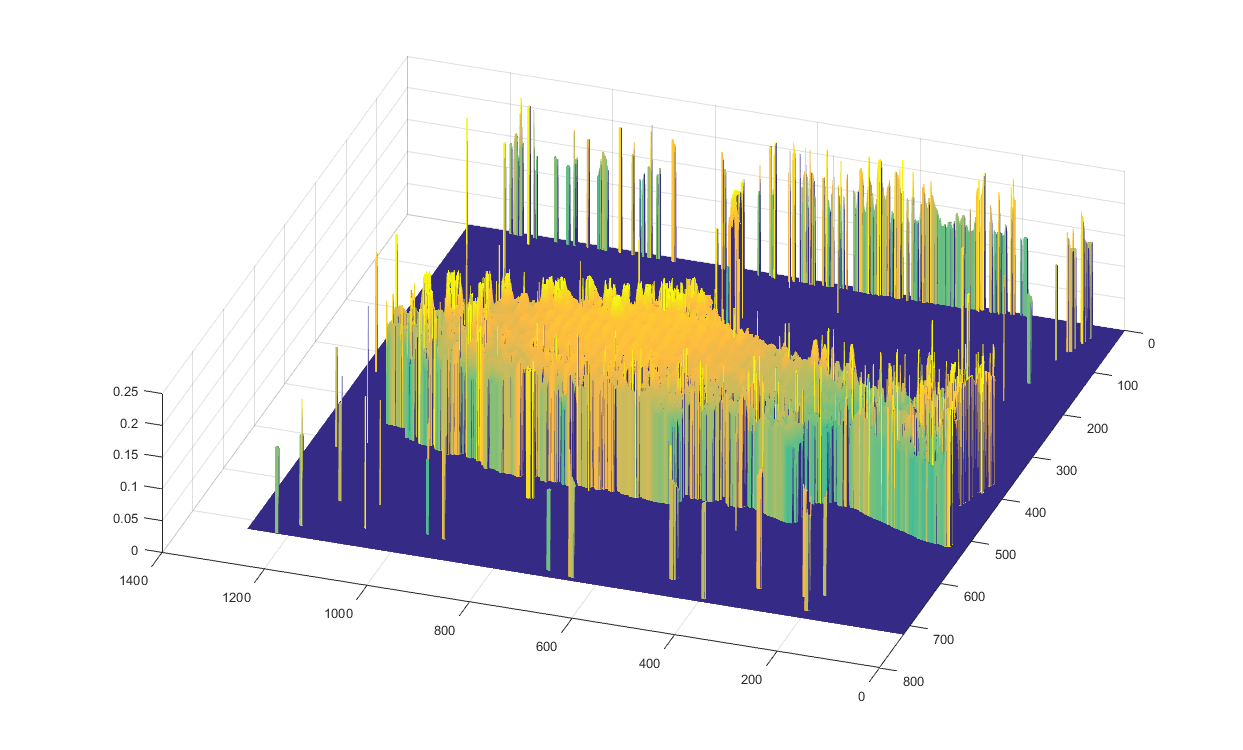
\includegraphics[width=.65\linewidth]{images/results/3D_plots/original_3D_63}
        \caption{Original depthmap} 
        \label{fig:3D_original_63}
    \end{subfigure}\hspace*{\fill}
    
    \medskip
    \begin{subfigure}{1\textwidth}
        \centering
        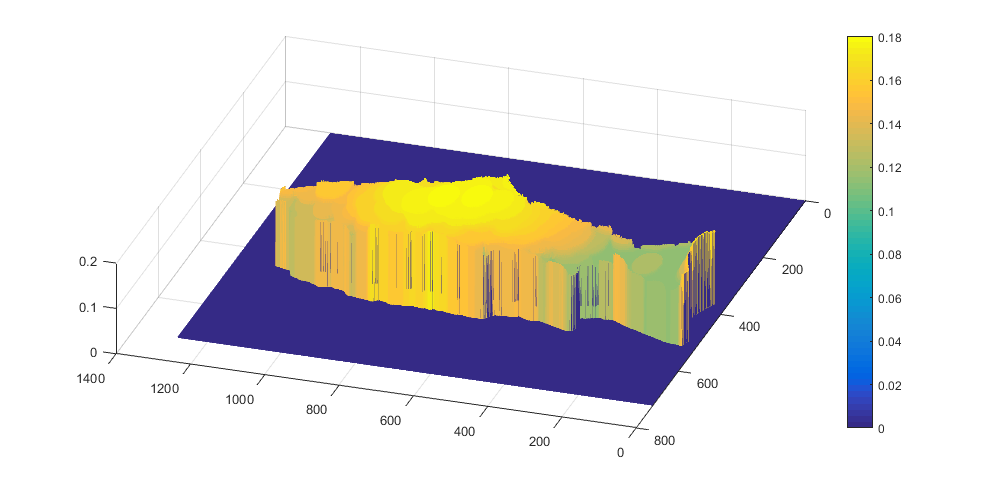
\includegraphics[width=.65\linewidth]{images/results/3D_plots/fixed_3D_63}
        \caption{Resulting depthmap} 
        \label{fig:3D_fixed_63}
    \end{subfigure}\hspace*{\fill}
    
    \medskip
    \begin{subfigure}{1\textwidth}
        \centering
        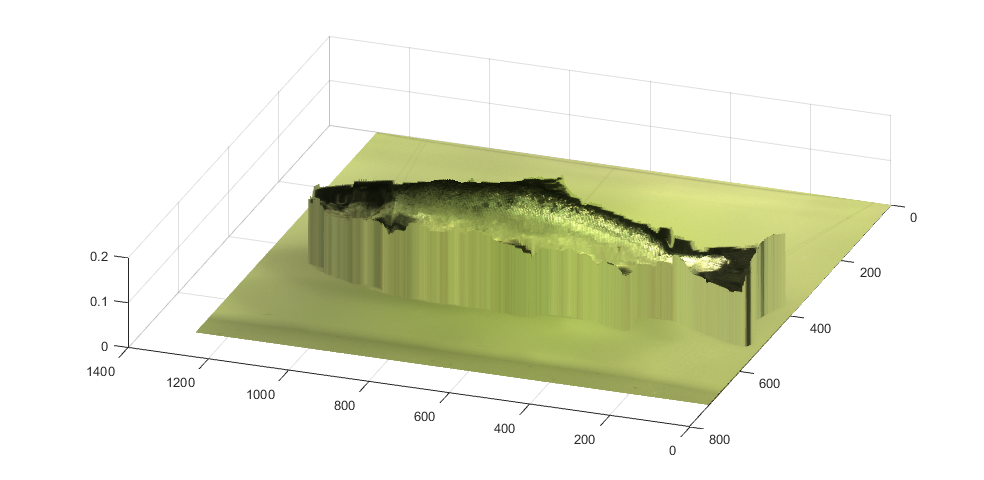
\includegraphics[width=.65\linewidth]{images/results/3D_plots/fixed_3D_fish_63}
        \caption{Resulting depthmap with image overlay} 
        \label{fig:3D_fixed_fish_63}
    \end{subfigure}\hspace*{\fill}
    \caption{3D plot of depthmap in MATLAB, number 563}
    \label{fig:3D_plot_63}
\end{figure}


\begin{figure}[H]
    \centering
    \begin{subfigure}{1\textwidth}
        \centering
        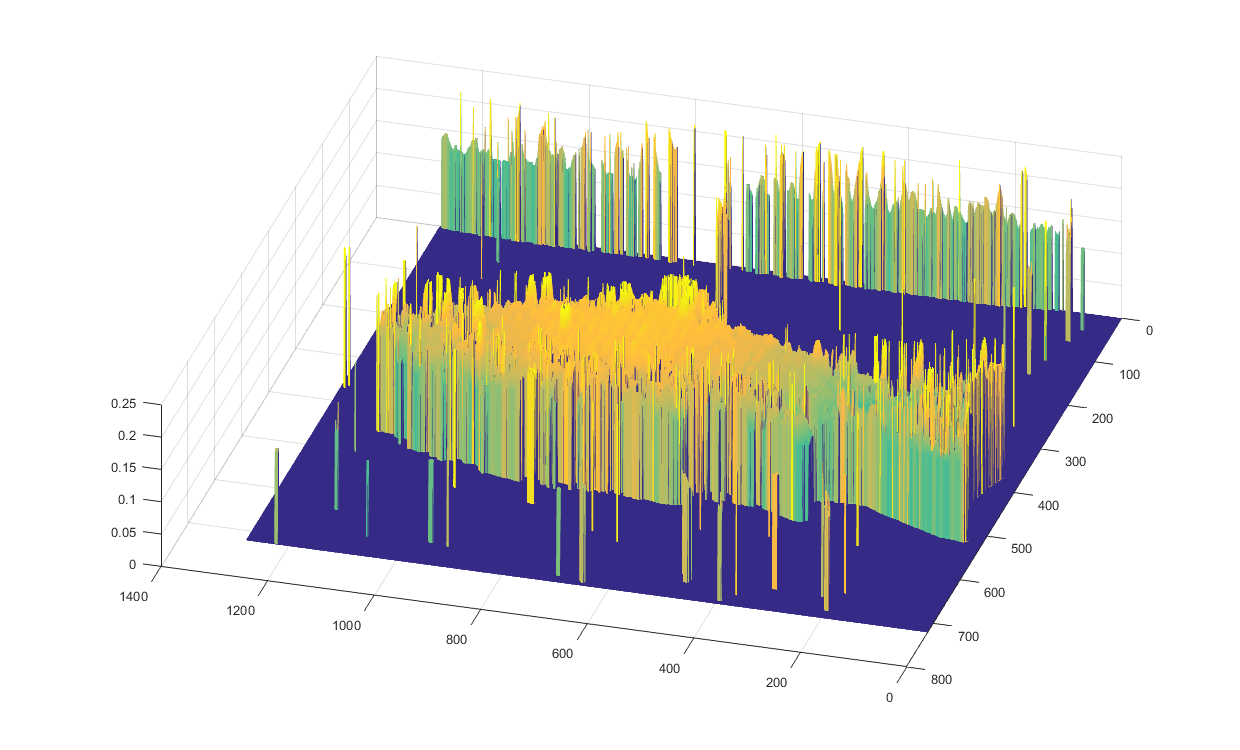
\includegraphics[width=.65\linewidth]{images/results/3D_plots/original_3D_87}
        \caption{Original depthmap} 
        \label{fig:3D_original_87}
    \end{subfigure}\hspace*{\fill}
    
    \medskip
    \begin{subfigure}{1\textwidth}
        \centering
        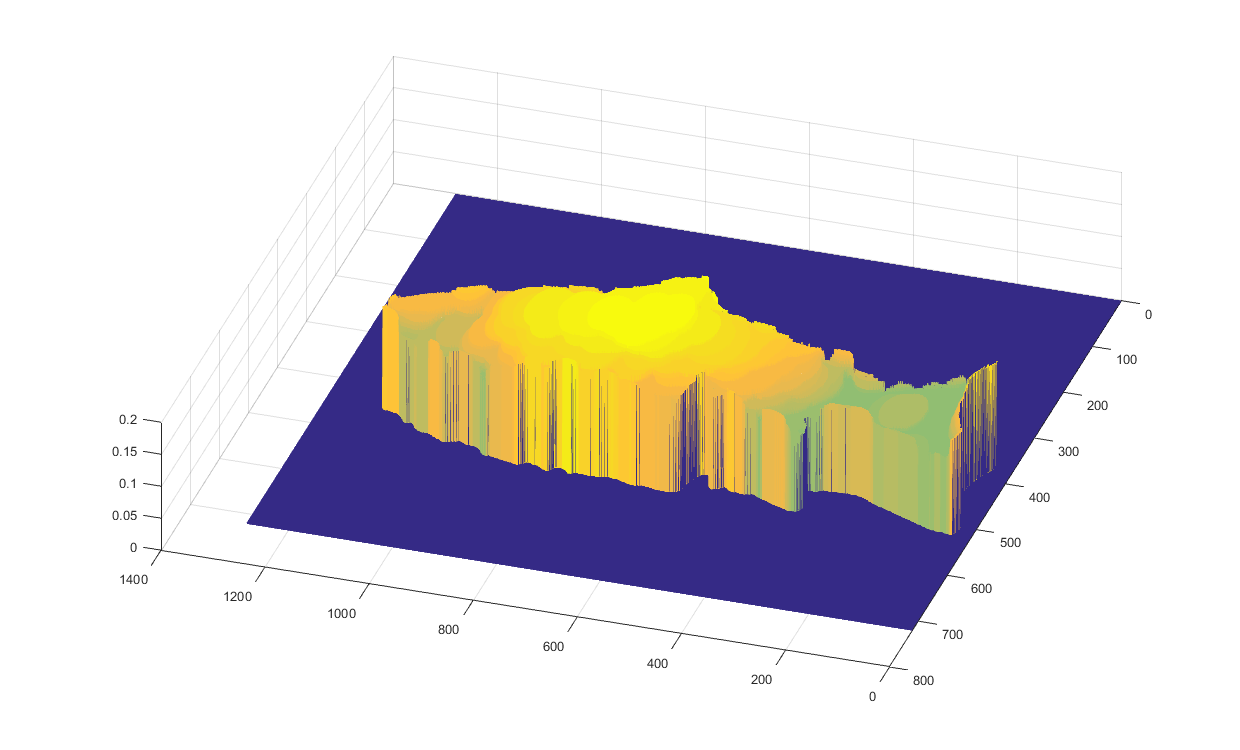
\includegraphics[width=.65\linewidth]{images/results/3D_plots/fixed_3D_87}
        \caption{Resulting depthmap} 
        \label{fig:3D_fixed_87}
    \end{subfigure}\hspace*{\fill}
    
    \medskip
    \begin{subfigure}{1\textwidth}
        \centering
        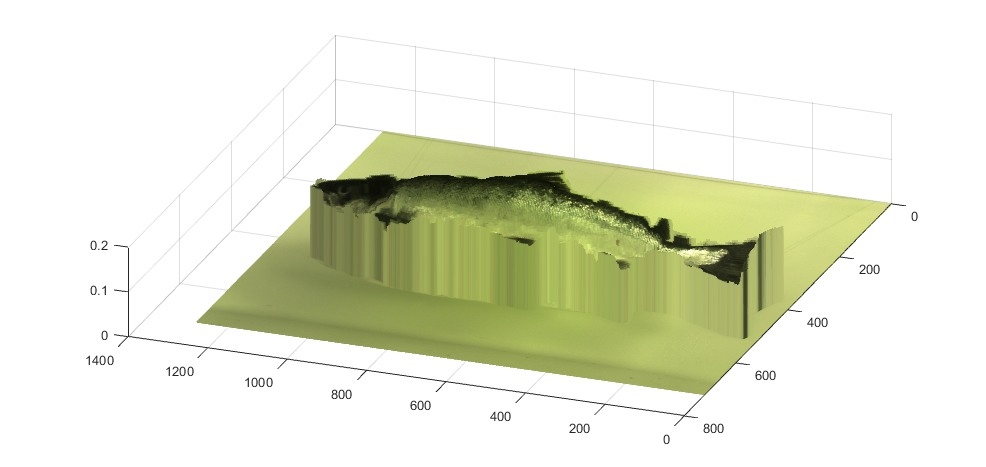
\includegraphics[width=.65\linewidth]{images/results/3D_plots/fixed_3D_fish_87}
        \caption{Resulting depthmap with image overlay} 
        \label{fig:3D_fixed_fish_87}
    \end{subfigure}\hspace*{\fill}
    \caption{3D plot of depthmap in MATLAB, number 587}
    \label{fig:3D_plot_87}
\end{figure}



\subsection{Noise}

It is seen from the noisy images that it has almost no effect on the result, still if the concentration of particles is high. This shows that the algorithm is robust and will work in most particle conditions as long as the light settings remains the same and the distance to the fish is within some boundaries.

With extreme particle conditions the depthmap looses to much depth information from the fish, and the contour will not be exact. This is though under such extreme particle conditions that it is not reasonable to believe that such conditions will occur in real life.


\subsection{Depth data preservation}

To ensure that the correct depth data from the depthmap is not changed in the enhanced depthmap, MATLAB plots is provided for one row of the depthmap along the fish. See figure \ref{fig:sectional} and \ref{fig:row_plot}. This plot shows the intensity values from the depthmap images, the original (red line) and the enhanced (blue line). The fishes head is to the right and its tale to the left. From the red line it is easy to see that most error on the original depthmap is found at the tail and the head, while the depth data along the middle of the fish is reasonable. From figure \ref{fig:plot1} it is also seen that the correct depth data is preserved and that the added data for the "holes" is within reason. It is though clear that there is still room for improvement for filling in depth data at the head and tail. 

\begin{figure}[h]
    \centering
    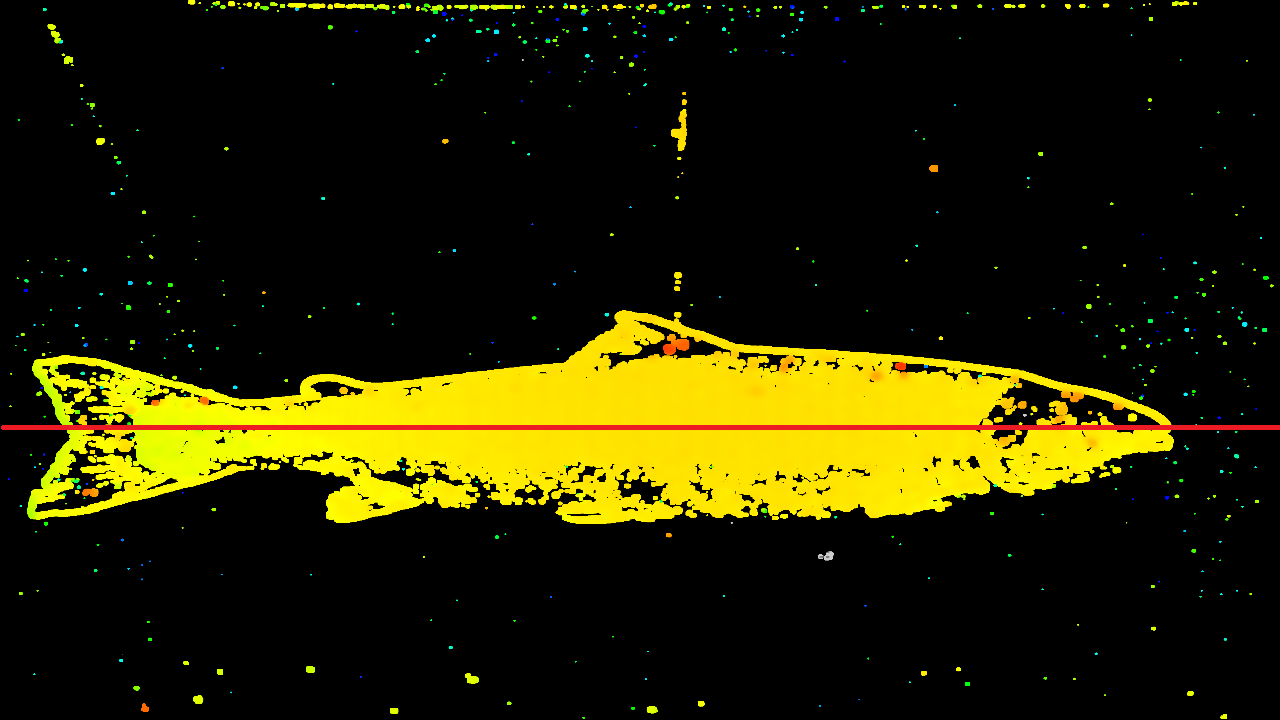
\includegraphics[width=.7\linewidth]{images/results/sectional}
    \caption{Plotted row}
    \label{fig:sectional}
\end{figure}


\begin{figure}[h]
    \centering
    \begin{subfigure}{1\textwidth}
        \centering
        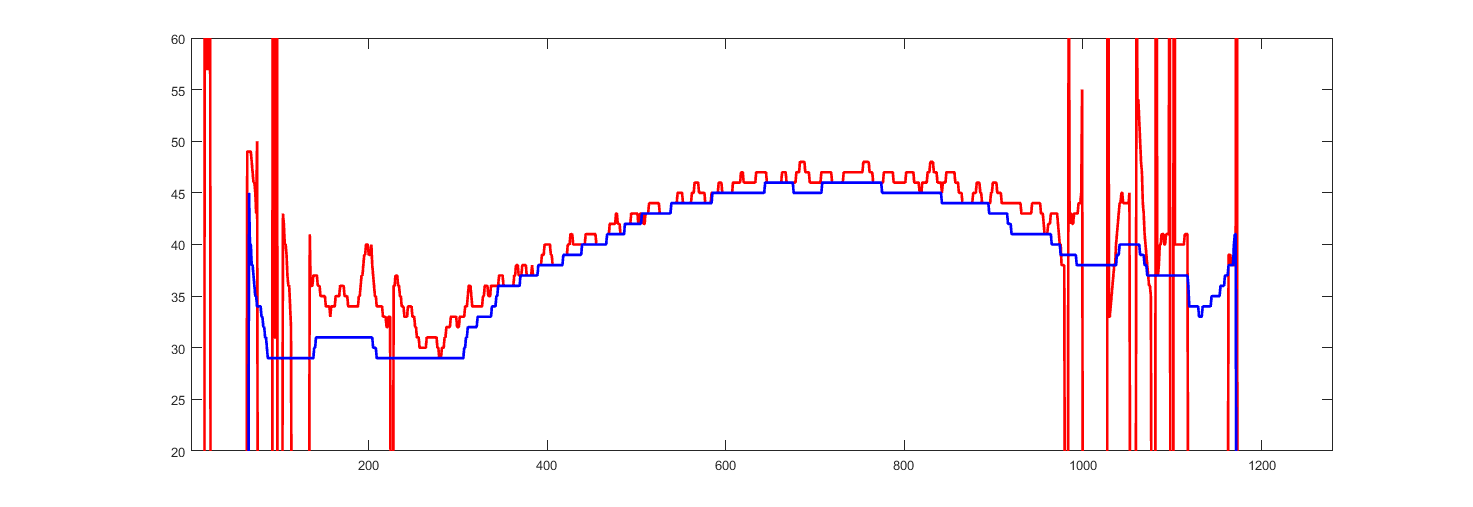
\includegraphics[width=1\linewidth]{images/results/plot_row}
        \caption{Plot of one row from the depthmap} 
        \label{fig:plot1}
    \end{subfigure}\hspace*{\fill}
    
    \medskip
    \begin{subfigure}{1\textwidth}
        \centering
        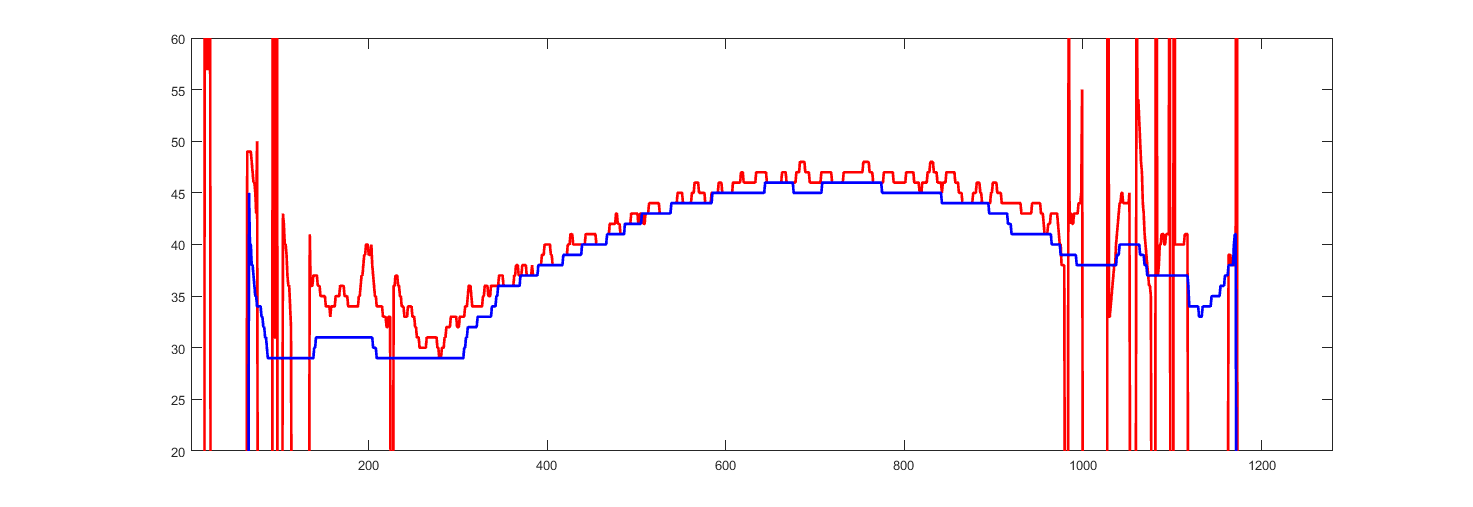
\includegraphics[width=1\linewidth]{images/results/plot_zoomed}
        \caption{Plot of one row from the depthmap, zoomed in} 
        \label{fig:plot2}
    \end{subfigure}\hspace*{\fill}
    \caption{Plot of depth information}
    \label{fig:row_plot}
\end{figure}


